% §5 Evaluation - ~1 page including 1 figure, 1 table. v0 draft.
\label{sec:eval}

\subsection{Headline results}
On the post-fix run, the \texttt{+position} router variant achieves \textbf{51 / 53 = 96.2\%} overall routing accuracy. Restricted to atomic tasks routed through the Reflexer, \textbf{32 / 35 = 91.4\%} of emitted commands match the gold regex; the three failures are all \texttt{caldav\_add} variants sharing one template-ordering issue. For composite tasks, \textbf{12 / 12} are routed to the correct composite; gold-command verification for the composite path is currently unavailable due to a benchmark-instrumentation gap (\S\ref{sec:disc}). All four out-of-distribution prompts are correctly identified as no-route. End-to-end outcome success is not reported because backend availability dominates the signal at this scale.

\subsection{Routing A/B}
Table~\ref{tab:ab} summarises overall accuracy across the five router variants; Fig.~\ref{fig:ab} breaks accuracy down by category. The position bonus is the sole driver of the improvement: \texttt{baseline}, \texttt{+laplace}, and \texttt{+margin} all score $46 / 53 = 86.8\%$, while \texttt{+position} and \texttt{all\_combined} both score $51 / 53 = 96.2\%$, a $+9.4$~pp gain. The gain is concentrated in two categories: \emph{v1\_collision\_regression} ($3 \to 6$) and \emph{atomic\_easy} ($17 \to 19$). On categories where the baseline already scored 100\% (composites, real-world, off-distribution), no variant changes the result. Laplace smoothing and margin gating do not change accuracy on this test set but, by construction, repair the failure modes documented in \S\ref{sec:disc}; their accuracy-neutrality is itself a positive result, since the safety nets do not regress correct routing.

\begin{table}[t]
  \centering
  \caption{Router A/B: overall accuracy on $n{=}53$ tasks.}
  \label{tab:ab}
  \small
  \begin{tabular}{lcc}
    \toprule
    Variant & Correct / Total & Accuracy \\
    \midrule
    baseline       & 46 / 53 & 86.8\% \\
    \texttt{+laplace}    & 46 / 53 & 86.8\% \\
    \texttt{+margin}     & 46 / 53 & 86.8\% \\
    \texttt{+position}   & \textbf{51 / 53} & \textbf{96.2\%} \\
    all\_combined   & \textbf{51 / 53} & \textbf{96.2\%} \\
    \bottomrule
  \end{tabular}
\end{table}

\begin{figure}[t]
  \centering
  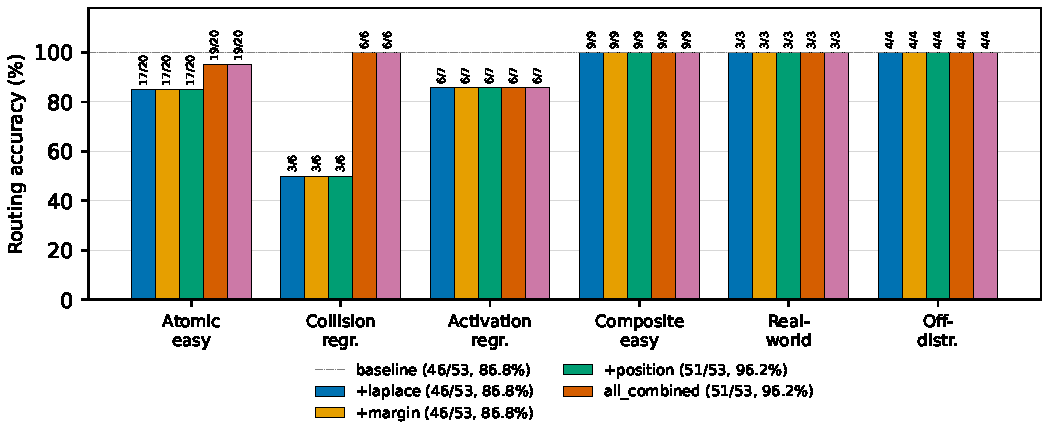
\includegraphics[width=\columnwidth]{figures/fig2_router_ab.pdf}
  \caption{Per-category routing accuracy for the five router variants on $n{=}53$ tasks. The position bonus delivers the entire 9.4~pp improvement; gains are concentrated in the atomic-easy and collision-regression categories.}
  \label{fig:ab}
\end{figure}

\subsection{Latency}
On the routed path the Reflexer is roughly an order of magnitude faster than the Thinker. Measured real LLM latency for the Reflexer ($n{=}35$ atomic tasks) is \textbf{395\,ms} median (p95 1130\,ms, max 1724\,ms), against a Thinker per-task total time ($n{=}38$, dry stub) of \textbf{4556\,ms} median (p95 76\,s, max 92\,s), a $\sim$11.5$\times$ median speedup. Because the Thinker total time includes dry-stub tool overhead, this is an end-to-end comparison rather than a like-for-like single-call measurement, but the order-of-magnitude gap is robust to that caveat.

\subsection{Three deployment findings}
Three named failure modes emerged in pilot runs, each repaired in the post-fix configuration and grounded in a before/after measurement on the 53-task suite. First, \emph{stats poisoning}: the \texttt{caldav\_list} success rate was driven below the routing threshold because transient backend rejections were counted as pattern failures; a Laplace prior together with a \texttt{command\_was\_wrong} heuristic that separates backend faults from pattern faults restored five calendar tasks. Second, \emph{composite hijack}: a fully-specified request such as ``schedule a meeting Sync 10:00 to 10:30'' was captured by a composite intended for under-specified meetings, because the composite trigger was too greedy on the verb ``schedule''; a negative lookahead on an explicit clock time corrected two tasks. Third, \emph{position-weighted scoring}: calendar phrases lacking the literal word ``calendar'' lost to weakly-tied sibling patterns under even success-rate scoring, and the first-window position bonus $b_{\text{pos}}=0.15$ delivered the $+9.4$~pp overall gain.
